\section{Ejercicio 1: Crear relaciones - Tarea 2: Relaciones manuales} 

\begin{enumerate}[1.]
	\item En la Ventana de Power BI Desktop, click en Obtener Datos (Get Data) y luego en Excel. Abrir el archivo Adventure Works Product Categories.xlsx. En el cuadro de dialogo Explorador (Navigator), seleccionar las hojas DimProductCategory, and
DimProductSubcategory, y luego hacer click en Cargar (Load).
	
	\begin{center}
	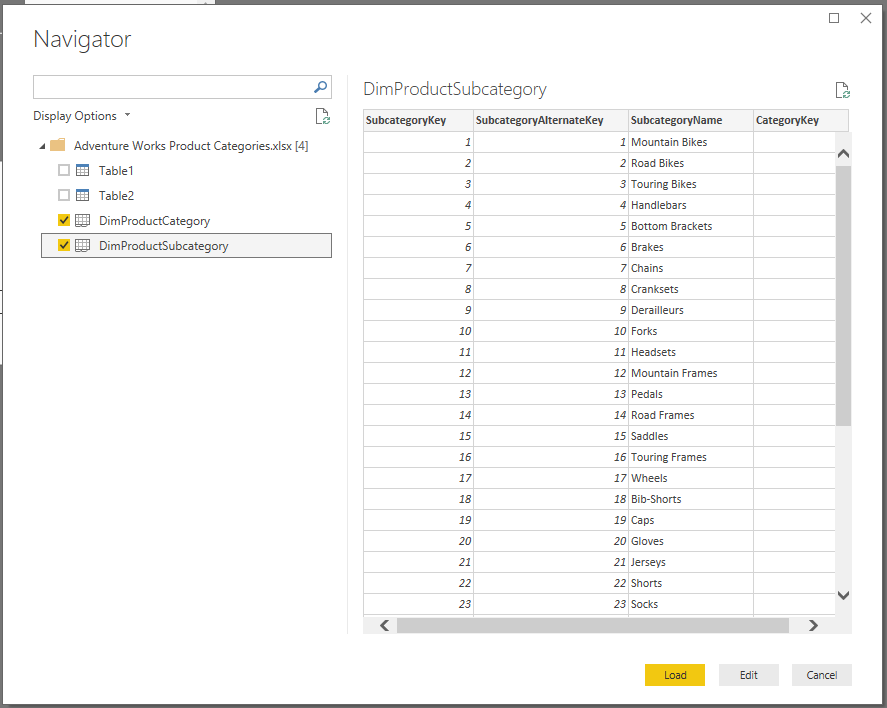
\includegraphics[width=11cm]{./Imagenes/21} 
	\end{center}

	\item En el panel de Relaciones, revisar la relación que Power BI ha creado entre las dos tablas.
 Hacer click en la línea de la relación entre DimProductCategory, y DimProductSubcategory, y seleccionar
Eliminar (Delete). En el cuadro de dialogo Eliminar relación (Delete Relationship), hacer click en Borrar (Delete).

	

	\begin{center}
	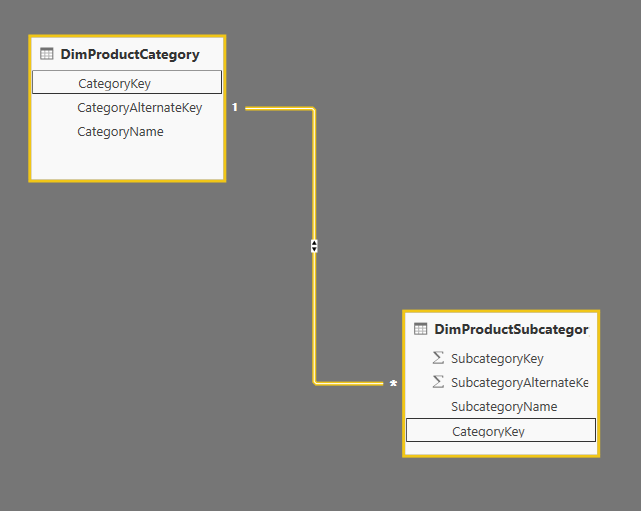
\includegraphics[width=9cm]{./Imagenes/22} 
	\end{center}

	\item Arrastrar la columna CategoryKey en la tabla DimProductSubcategory a la columna Category en la tabla
DimProductCategory, para crear una relación Muchos a uno (Many to One (*:1)), y una dirección de filtro
cruzado (Cross filter direction) en ambos

	
	\begin{center}
	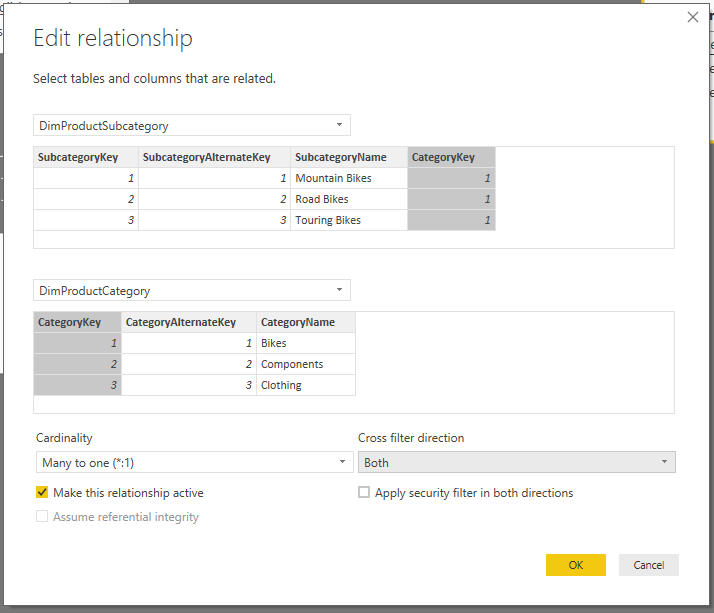
\includegraphics[width=11cm]{./Imagenes/23} 
	\end{center}


	\item En la tabla DimProduct, arrastrar la columna ProductSubcategoryKey a la columna SubcategoryKey en la tabla DimProductSubcategory, para crear una relación de Muchos a Uno (Many to One (*:1)), y una dirección de filtro cruzado (Cross filter direction) en ambos.
	
	\begin{center}
	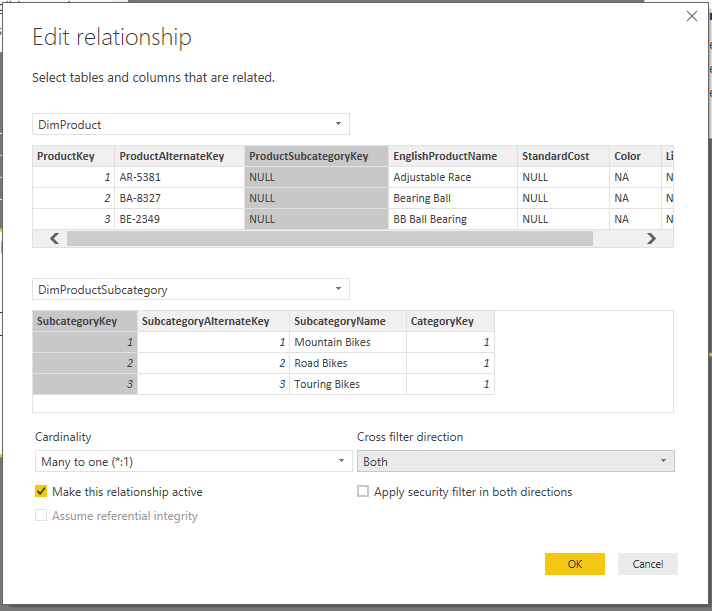
\includegraphics[width=11cm]{./Imagenes/24} 
	\end{center}

	\item Hacer click en Guardar
	
	\begin{center}
	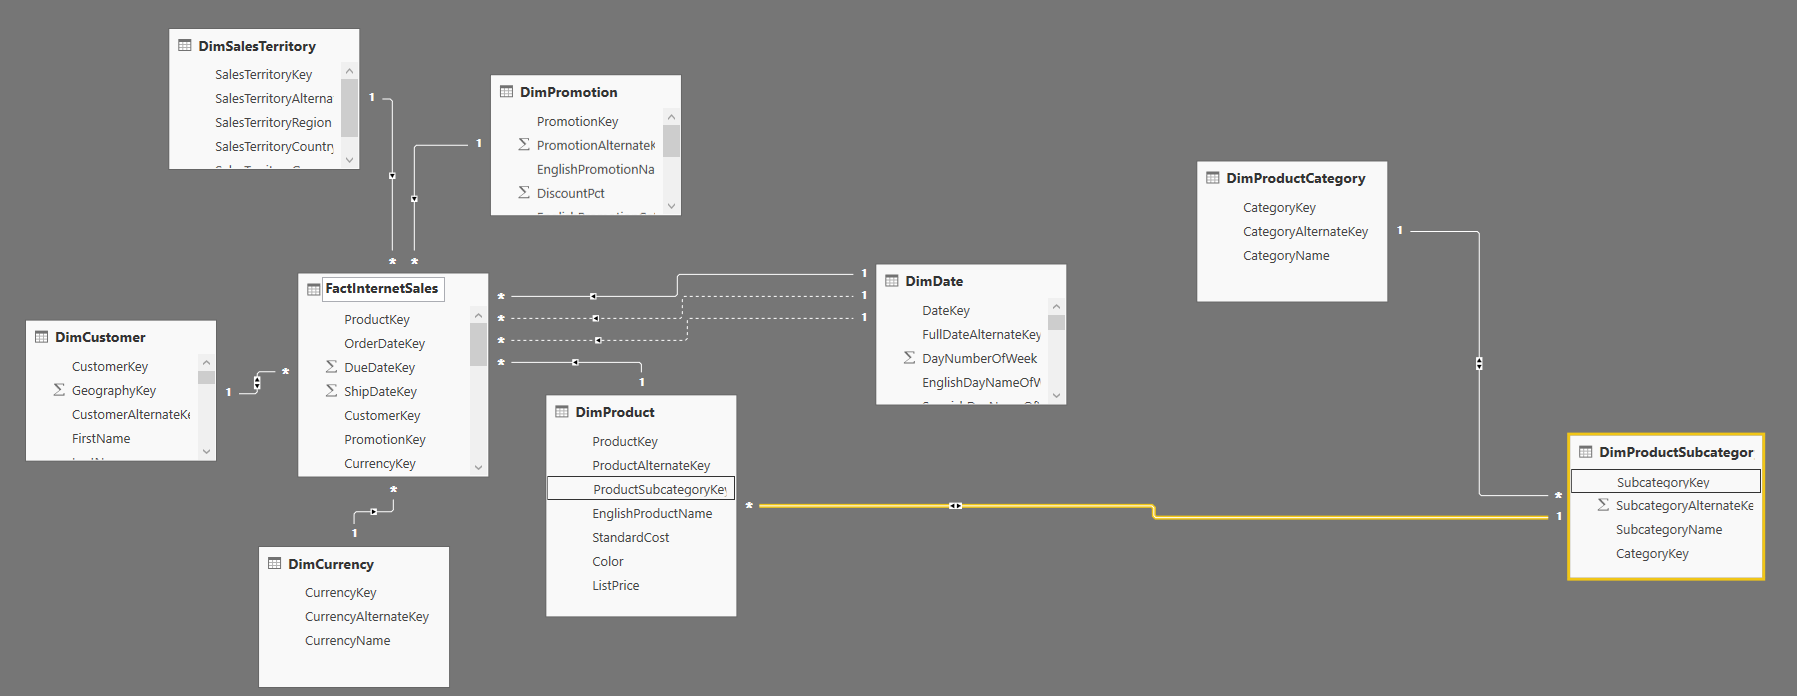
\includegraphics[width=18cm]{./Imagenes/25} 
	\end{center}

\end{enumerate}


